% ==========================================================
% ENTREGABLE 2 - INTELIGENCIA DE NEGOCIOS
% Arquitectura de Datos Técnica y Modelo Dimensional
% Universidad Estatal Península de Santa Elena
% ==========================================================

\documentclass[12pt,a4paper]{article}

% ==========================================================
% PAQUETES
% ==========================================================
\usepackage[utf8]{inputenc}
\usepackage[T1]{fontenc}
\usepackage[spanish,es-tabla]{babel}
\usepackage[top=2.5cm,bottom=2.5cm,left=2.5cm,right=2.5cm]{geometry}
\usepackage{graphicx}
\usepackage[table]{xcolor}
\usepackage{titlesec}
\usepackage{enumitem}
\usepackage{tabularx}
\usepackage{booktabs}
\usepackage{longtable}
\usepackage{array}
\usepackage{float}
\usepackage{hyperref}
\usepackage{parskip}
\usepackage{pdflscape}

% ==========================================================
% COLORES Y ESTILO
% ==========================================================
\definecolor{primarygray}{gray}{0.35}
\definecolor{textblack}{gray}{0.0}
\definecolor{lightgray}{gray}{0.92}

\titleformat{\section}
{\color{primarygray}\Large\bfseries}
{\thesection.}
{0.5em}
{}

\titleformat{\subsection}
{\color{primarygray}\large\bfseries}
{\thesubsection.}
{0.5em}
{}

\hypersetup{
    colorlinks=true,
    linkcolor=textblack,
    urlcolor=primarygray,
    citecolor=primarygray
}

\renewcommand{\arraystretch}{1.25}
\setlength{\tabcolsep}{4pt}

\newcolumntype{P}[1]{>{\raggedright\arraybackslash}p{#1}}
\newcommand{\FactTabla}{\texttt{FactActividadAgenteIA}}

\begin{document}

% ==========================================================
% PORTADA
% ==========================================================
\begin{titlepage}
\centering
\vspace*{0.6cm}

\IfFileExists{upse.jpg}{
    \includegraphics[width=5cm]{upse.jpg}\\[0.5cm]
}{
    {\Large \textbf{UPSE}}\\[0.5cm]
}

{\Large \textbf{\textcolor{primarygray}{UNIVERSIDAD ESTATAL PENÍNSULA DE SANTA ELENA}}}\\[0.3cm]
{\large \textbf{Ingeniería de Software}}\\[0.1cm]
{\large Sexto Semestre}\\[1.2cm]

{\large \textbf{VI Inteligencia de Negocios}}\\[0.8cm]
{\LARGE \textbf{\textcolor{primarygray}{ENTREGABLE 2}}}\\[0.3cm]
{\Large Arquitectura de Datos Técnica y Modelo Dimensional}\\[1.2cm]

{\large \textbf{Título del Proyecto}}\\[0.4cm]

\begin{minipage}{0.92\textwidth}
\centering
\large
Plataforma de Inteligencia de Negocios para el análisis de tendencias, adopción y evolución de agentes de Inteligencia Artificial en el dominio del desarrollo de software mediante integración de datos heterogéneos durante el período 2023--2026
\end{minipage}

\vfill

{\textbf{Autores}}\\[0.2cm]
Damian Jesús Torres Cadena\\
Melanie Adriana Tomalá Merejildo\\
Jean Pierre Cedeño Andrade
\vfill
{\textbf{Docente:}}\\[0.2cm]
Ing: Anthony Pachay
\vfill


{\textbf{Período Académico}}\\
2026--1

\end{titlepage}

\tableofcontents
\newpage

% ==========================================================
\section{Arquitectura de Datos Técnica}

La arquitectura técnica del proyecto se estructura en capas para integrar fuentes heterogéneas relacionadas con agentes de Inteligencia Artificial aplicados al desarrollo de software. El flujo inicia con la extracción de datos desde APIs, técnicas de web scraping, archivos estructurados y encuesta académica; posteriormente, los datos pasan por una zona Raw, una zona Staging y finalmente se consolidan en un Data Warehouse dimensional para su explotación mediante dashboards.

\begin{figure}[H]
\centering
\IfFileExists{diagrama.png}{
    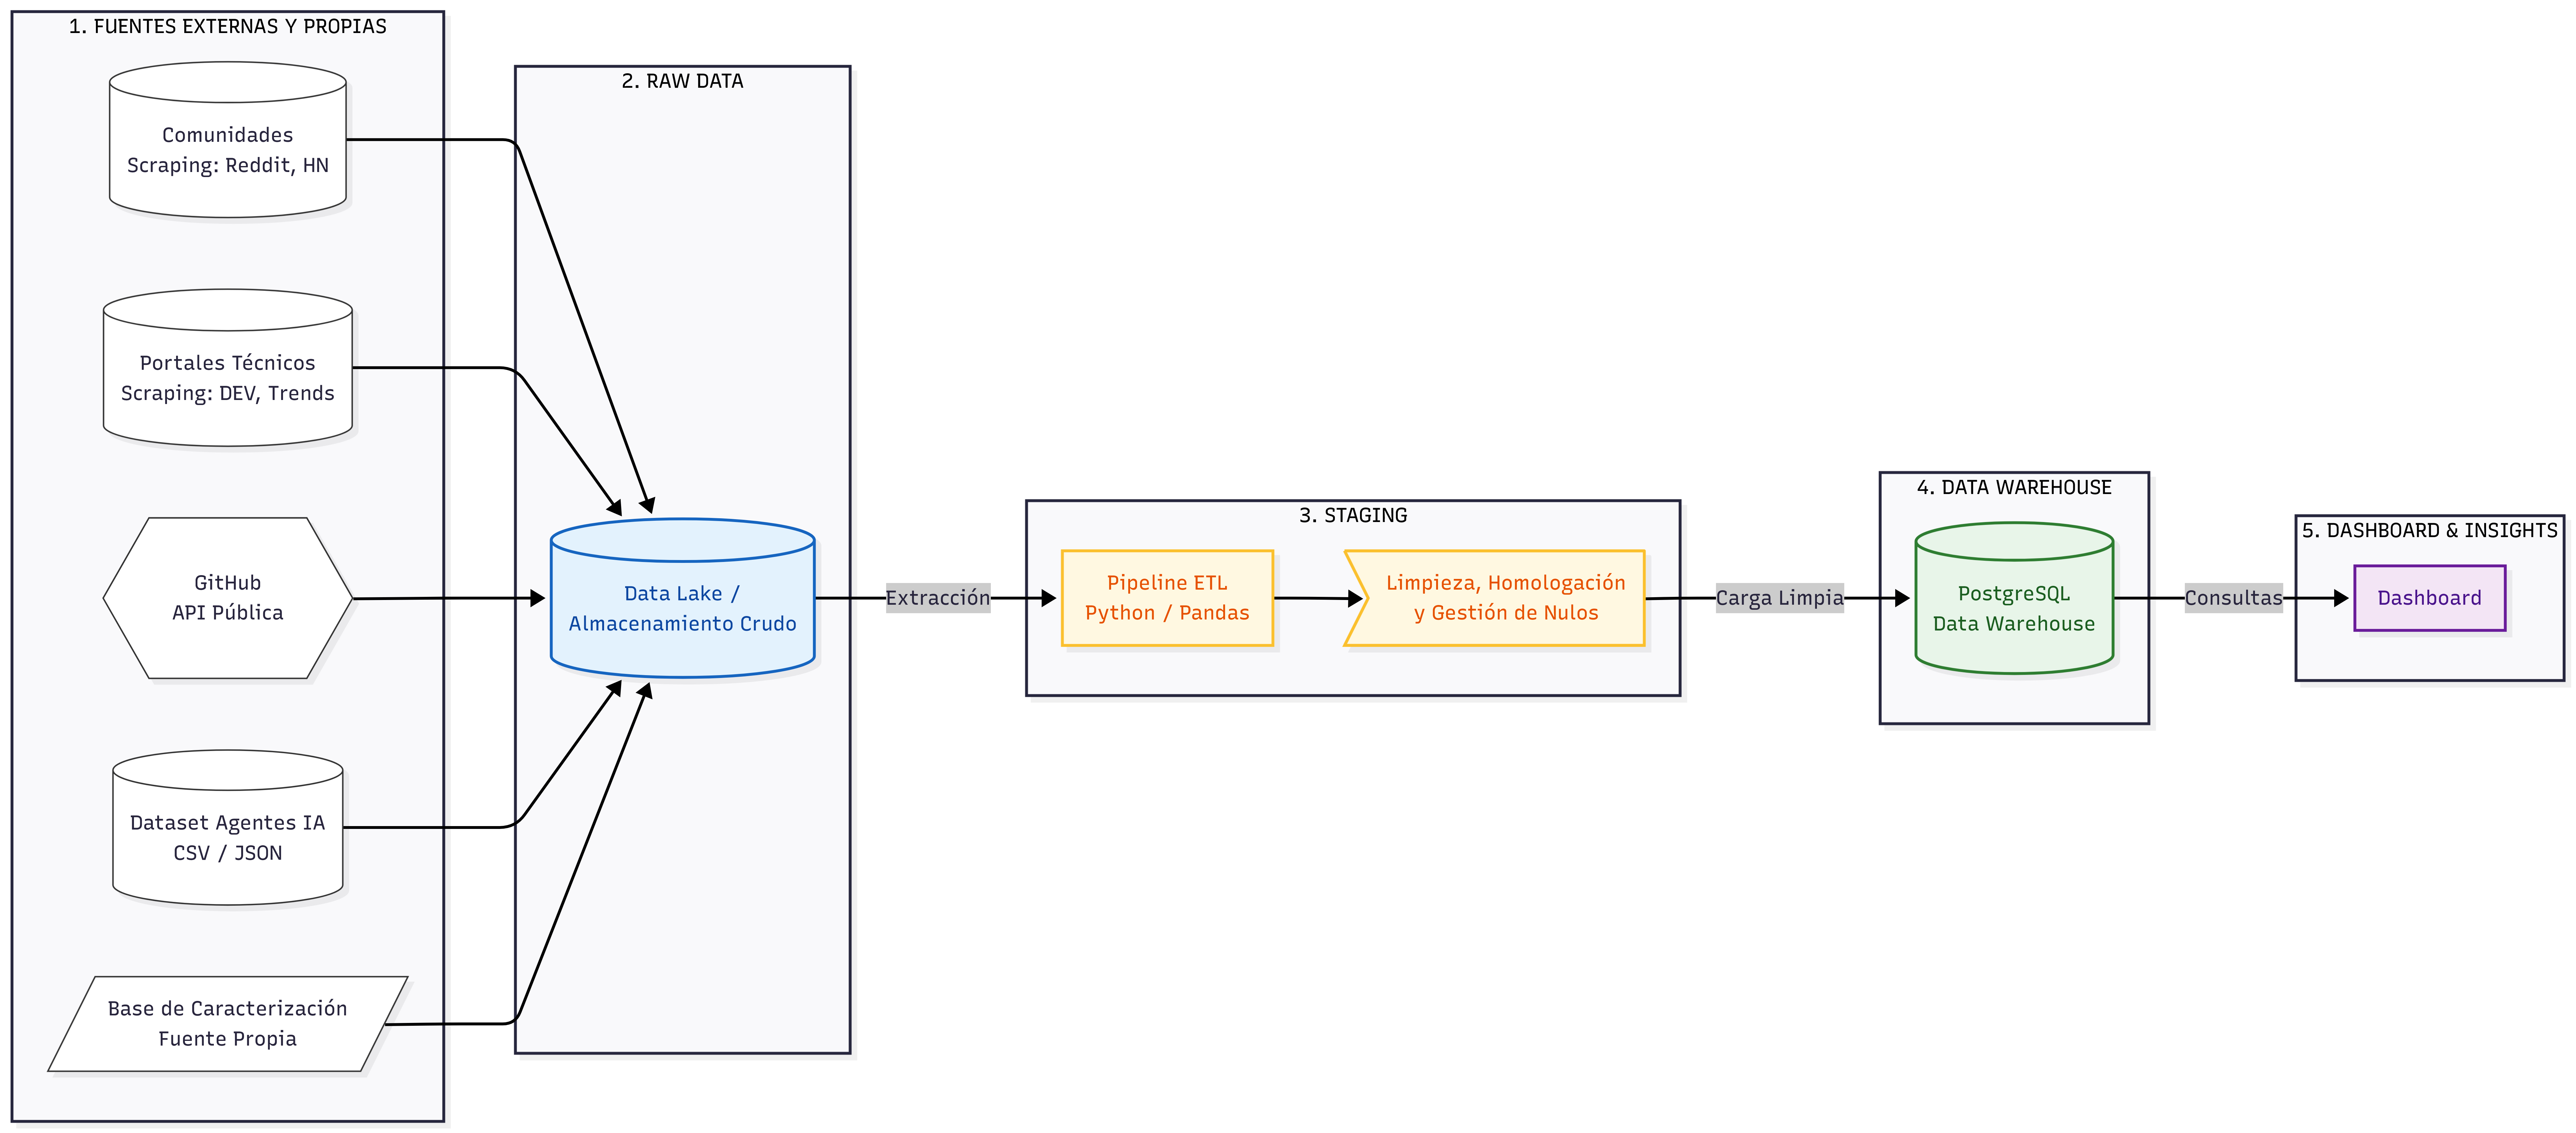
\includegraphics[width=0.95\textwidth]{diagrama.png}
}{
    \fbox{
        \begin{minipage}[c][7cm][c]{0.9\textwidth}
        \centering
        \textbf{Espacio reservado para el diagrama de arquitectura técnica}\\[0.3cm]
        Subir el archivo \texttt{diagrama.png} en la misma carpeta del archivo \texttt{.tex}.
        \end{minipage}
    }
}
\caption{Arquitectura técnica de datos para el análisis de agentes de Inteligencia Artificial}
\end{figure}

\begin{table}[H]
\centering
\small
\rowcolors{2}{gray!8}{white}
\begin{tabular}{|P{3.3cm}|P{5.3cm}|P{5.8cm}|}
\hline
\rowcolor{gray!25}
\textbf{Capa} & \textbf{Tecnologías / mecanismos} & \textbf{Función dentro de la arquitectura} \\ \hline
Orígenes de datos & GitHub API, Reddit, DEV Community, Hacker News, Google Trends, CSV/JSON, Encuesta UPSE & Proveer datos sobre actividad técnica, popularidad, menciones, producción técnica, innovación y adopción académica. \\ \hline
Extracción & Python, requests, pandas, BeautifulSoup, pytrends & Extraer datos desde APIs, scraping web, archivos estructurados y formularios exportados. \\ \hline
Zona Raw & Archivos JSON, CSV o Parquet & Conservar los datos originales sin transformación para trazabilidad histórica. \\ \hline
Zona Staging & PostgreSQL, esquema \texttt{staging}, scripts Python y SQL & Limpiar, validar, estandarizar nombres de agentes, homologar fuentes y preparar datos para el DW. \\ \hline
Data Warehouse & PostgreSQL, esquema \texttt{dw}, Star Schema & Almacenar información analítica mediante una tabla de hechos y dimensiones. \\ \hline
Capa BI & Dashboard principal y prototipo interactivo opcional & Visualizar KPIs de popularidad, adopción, actividad técnica, producción técnica e innovación mediante una capa de presentación analítica. \\ \hline
\end{tabular}
\caption{Capas técnicas de la arquitectura de datos}
\end{table}

% ==========================================================
\section{Modelo Dimensional}

\subsection{Declaración de Granularidad}

Cada fila dentro de la tabla de hechos \texttt{FactActividadAgenteIA} representará una medición atómica de actividad, popularidad, adopción o interacción asociada a un agente de Inteligencia Artificial, en una fecha específica, proveniente de una fuente identificable y vinculada a un ID de origen del registro.

La granularidad definida permite analizar la evolución temporal de cada agente de IA por fuente, plataforma y categoría, evitando un modelo OLTP transaccional y priorizando el análisis agregado mediante métricas cuantitativas.

\subsection{Matriz del Modelo de Hechos}

\small
\rowcolors{2}{gray!8}{white}

\begin{longtable}{|P{3.2cm}|P{2.7cm}|P{7cm}|P{2.2cm}|}
\hline
\rowcolor{gray!25}
\textbf{Campo Destino} & \textbf{Tipo SQL} & \textbf{Descripción Funcional} & \textbf{Rol Estructural} \\ \hline
\endfirsthead

\hline
\rowcolor{gray!25}
\textbf{Campo Destino} & \textbf{Tipo SQL} & \textbf{Descripción Funcional} & \textbf{Rol Estructural} \\ \hline
\endhead

id\_hecho & SERIAL / INT & Clave primaria surrogada auto-incremental de la tabla de hechos. & PK \\ \hline
id\_tiempo & INT & Clave foránea hacia la dimensión de tiempo. & FK \\ \hline
id\_agente & INT & Clave foránea hacia la dimensión de agentes de IA. & FK \\ \hline
id\_fuente & INT & Clave foránea hacia la dimensión de fuentes de datos. & FK \\ \hline
id\_plataforma & INT & Clave foránea hacia la dimensión de plataformas digitales. & FK \\ \hline
id\_categoria & INT & Clave foránea hacia la dimensión de categorías analíticas. & FK \\ \hline
id\_origen\_registro & VARCHAR(120) & Identificador original del registro en la fuente de procedencia. & Degenerada \\ \hline
cantidad\_menciones & INT & Número de menciones detectadas del agente en la fuente. & Métrica \\ \hline
cantidad\_interacciones & INT & Total de interacciones asociadas al registro: comentarios, votos, reacciones o respuestas. & Métrica \\ \hline
score\_popularidad & DECIMAL(10,2) & Valor normalizado de popularidad del agente según la fuente analizada. & Métrica \\ \hline
stars\_github & INT & Número de estrellas obtenidas por repositorios relacionados con el agente. & Métrica \\ \hline
forks\_github & INT & Número de forks en repositorios asociados al agente. & Métrica \\ \hline
issues\_abiertos & INT & Número de issues abiertos en repositorios relacionados. & Métrica \\ \hline
releases & INT & Cantidad de versiones o releases publicados por período. & Métrica \\ \hline
indice\_adopcion & DECIMAL(5,2) & Porcentaje normalizado de adopción del agente según encuesta o fuente estructurada. & Métrica \\ \hline
indice\_innovacion & DECIMAL(5,2) & Indicador calculado para medir aparición, novedad o crecimiento del agente por período. & Métrica \\ \hline
sentimiento\_promedio & DECIMAL(5,2) & Valor promedio de percepción textual asociado al agente, en escala de -1 a 1. & Métrica \\ \hline
fecha\_carga & TIMESTAMP & Fecha y hora de carga del registro al Data Warehouse. & Auditoría \\ \hline

\caption{Matriz del modelo de hechos}
\end{longtable}

\normalsize

% ==========================================================
\section{Justificación de la Topología del Esquema}

\begin{table}[H]
\centering
\small
\rowcolors{2}{gray!8}{white}
\begin{tabular}{|P{4cm}|P{3.4cm}|P{3.4cm}|P{3.4cm}|}
\hline
\rowcolor{gray!25}
\textbf{Criterio Evaluativo} & \textbf{Star Schema (Estrella)} & \textbf{Snowflake (Copo de Nieve)} & \textbf{Galaxy Schema (Galaxia)} \\ \hline
Rendimiento Joins & Alto & Medio & Alto \\ \hline
Redundancia & Alta & Baja & Media \\ \hline
Complejidad & Baja & Media & Alta \\ \hline
Facilidad para BI & Alta & Media & Media \\ \hline
Mantenimiento académico & Alto & Medio & Bajo \\ \hline
¿Aplica al caso? & Sí & No & No \\ \hline
\end{tabular}
\caption{Comparación de topologías dimensionales}
\end{table}

Se selecciona un \textbf{Star Schema} porque el proyecto requiere analizar métricas agregadas de popularidad, adopción, actividad técnica e innovación de agentes de IA con consultas simples y eficientes. Esta topología facilita la conexión con una capa de dashboard principal, reduce la complejidad del modelo y evita diseñar una base OLTP normalizada. El enfoque Snowflake no se prioriza porque aumentaría la cantidad de joins sin aportar un beneficio relevante para este hito. El enfoque Galaxy tampoco aplica, debido a que el modelo actual se centra en una tabla de hechos principal.

% ==========================================================
\section{Diccionario de Datos y Trazabilidad}

% Ajuste de formato: se amplía el área útil de la página en modo horizontal
% y se reducen los espacios internos de la tabla para evitar solapamientos.
\clearpage
\newgeometry{left=1.3cm,right=1.3cm,top=1.5cm,bottom=1.5cm}
\begin{landscape}
\begingroup
\scriptsize
\setlength{\tabcolsep}{2.2pt}
\renewcommand{\arraystretch}{1.18}
\rowcolors{2}{gray!8}{white}

\begin{longtable}{|P{3.55cm}|P{3.05cm}|P{2.35cm}|P{4.00cm}|P{3.95cm}|P{4.95cm}|P{3.05cm}|}
\hline
\rowcolor{gray!25}
\textbf{Tabla DW} & \textbf{Campo DW} & \textbf{Tipo} & \textbf{Regla / Valores} & \textbf{Atributo Staging} & \textbf{Transformación} & \textbf{Fuente Origen} \\ \hline
\endfirsthead

\hline
\rowcolor{gray!25}
\textbf{Tabla DW} & \textbf{Campo DW} & \textbf{Tipo} & \textbf{Regla / Valores} & \textbf{Atributo Staging} & \textbf{Transformación} & \textbf{Fuente Origen} \\ \hline
\endhead

DimTiempo & id\_tiempo & INT & PK, formato AAAAMMDD & stg\_fecha & Conversión de fecha a clave numérica. & Todas las fuentes \\ \hline
DimTiempo & fecha & DATE & Fecha válida & stg\_fecha & Conversión a tipo DATE. & Todas las fuentes \\ \hline
DimTiempo & anio & SMALLINT & 2023--2026 & stg\_fecha & Extracción del año. & Todas las fuentes \\ \hline
DimTiempo & trimestre & SMALLINT & 1--4 & stg\_fecha & Cálculo del trimestre. & Todas las fuentes \\ \hline
DimTiempo & mes & SMALLINT & 1--12 & stg\_fecha & Extracción del mes. & Todas las fuentes \\ \hline
DimTiempo & nombre\_mes & VARCHAR(20) & Enero--Diciembre & stg\_fecha & Conversión del número de mes a nombre. & Todas las fuentes \\ \hline
DimTiempo & semana & SMALLINT & 1--53 & stg\_fecha & Cálculo de semana del año. & Todas las fuentes \\ \hline

DimFuente & id\_fuente & INT & PK auto-incremental & stg\_fuente & Generación de clave surrogada. & Todas las fuentes \\ \hline
DimFuente & nombre\_fuente & VARCHAR(60) & GitHub, Reddit, DEV, Hacker News, Google Trends, CSV/JSON, Encuesta UPSE & stg\_fuente & Estandarización del nombre de la fuente. & Todas las fuentes \\ \hline
DimFuente & tipo\_fuente & VARCHAR(40) & API, Scraping, Archivo, Encuesta & stg\_tipo\_fuente & Clasificación del mecanismo de origen. & Todas las fuentes \\ \hline
DimFuente & mecanismo\_extraccion & VARCHAR(80) & requests, BeautifulSoup, pytrends, carga CSV & stg\_mecanismo & Registro del mecanismo de extracción utilizado. & Scripts Python \\ \hline

DimAgente & id\_agente & INT & PK auto-incremental & stg\_nombre\_agente & Generación de clave surrogada. & Dataset CSV/JSON \\ \hline
DimAgente & nombre\_agente & VARCHAR(80) & Nombre oficial del agente & stg\_nombre\_agente & Estandarización de variantes del nombre. & Dataset CSV/JSON, GitHub, comunidades \\ \hline
DimAgente & desarrollador & VARCHAR(100) & Organización o proveedor & stg\_desarrollador & Normalización de nombre de empresa o comunidad. & Dataset CSV/JSON \\ \hline
DimAgente & modelo\_base & VARCHAR(100) & GPT, Claude, Gemini, modelo propio u otro & stg\_modelo\_base & Homologación de modelo base. & Dataset CSV/JSON \\ \hline
DimAgente & categoria\_agente & VARCHAR(80) & Asistente, editor IA, agente autónomo, herramienta QA & stg\_categoria\_agente & Clasificación por categoría funcional. & Dataset CSV/JSON \\ \hline
DimAgente & fecha\_lanzamiento & DATE & Fecha válida o NULL & stg\_fecha\_lanzamiento & Conversión a tipo DATE. & Dataset CSV/JSON \\ \hline

DimPlataforma & id\_plataforma & INT & PK auto-incremental & stg\_plataforma & Generación de clave surrogada. & Todas las fuentes \\ \hline
DimPlataforma & nombre\_plataforma & VARCHAR(80) & VS Code, JetBrains IDEs, Terminal/CLI, API/SDK, Web, cloud & dim\_nombre\_plataforma & Inferencia desde metadata, contexto o formato inequívoco del agente. & Todas las fuentes \\ \hline
DimPlataforma & tipo\_plataforma & VARCHAR(60) & Entorno de desarrollo, CLI, interfaz programática, aplicación web, cloud & dim\_tipo\_plataforma & Clasificación del entorno de ejecución o integración. & Todas las fuentes \\ \hline

DimCategoria & id\_categoria & INT & PK auto-incremental & stg\_categoria & Generación de clave surrogada. & Todas las fuentes \\ \hline
DimCategoria & nombre\_categoria & VARCHAR(80) & Popularidad, adopción, actividad técnica, producción técnica, innovación & stg\_categoria & Homologación de categoría analítica. & Todas las fuentes \\ \hline
DimCategoria & descripcion & VARCHAR(200) & Descripción funcional de la categoría & stg\_categoria & Asignación de descripción según regla de negocio. & Diccionario interno \\ \hline

\FactTabla & id\_hecho & SERIAL / INT & PK auto-incremental & No aplica & Generación automática al insertar el registro. & DW \\ \hline
\FactTabla & id\_tiempo & INT & FK válida en DimTiempo & stg\_fecha & Búsqueda de clave en DimTiempo. & Todas las fuentes \\ \hline
\FactTabla & id\_agente & INT & FK válida en DimAgente & stg\_nombre\_agente & Búsqueda de clave por nombre estandarizado del agente. & Todas las fuentes \\ \hline
\FactTabla & id\_fuente & INT & FK válida en DimFuente & stg\_fuente & Búsqueda de clave por fuente homologada. & Todas las fuentes \\ \hline
\FactTabla & id\_plataforma & INT & FK válida en DimPlataforma & dim\_nombre\_plataforma & Búsqueda de clave por entorno de ejecución o integración. & Todas las fuentes \\ \hline
\FactTabla & id\_categoria & INT & FK válida en DimCategoria & stg\_categoria & Clasificación según tipo de métrica y fuente. & Todas las fuentes \\ \hline
\FactTabla & id\_origen\_registro & VARCHAR(120) & ID original, URL o hash & stg\_id\_origen & Conservación del identificador original del registro. & Todas las fuentes \\ \hline
\FactTabla & cantidad\_menciones & INT & Mayor o igual a 0 & stg\_menciones & Conteo de apariciones del agente por período y fuente. & Reddit, DEV, Hacker News, Trends \\ \hline
\FactTabla & cantidad\_interacciones & INT & Mayor o igual a 0 & stg\_interacciones & Suma de comentarios, votos, reacciones o respuestas disponibles. & Reddit, DEV, Hacker News \\ \hline
\FactTabla & score\_popularidad & DECIMAL(10,2) & 0--100 & stg\_score\_trends & Normalización del interés relativo de búsqueda. & Google Trends \\ \hline
\FactTabla & stars\_github & INT & Mayor o igual a 0 & stg\_stars & Conversión a entero y validación de nulos. & GitHub API \\ \hline
\FactTabla & forks\_github & INT & Mayor o igual a 0 & stg\_forks & Conversión a entero y validación de nulos. & GitHub API \\ \hline
\FactTabla & issues\_abiertos & INT & Mayor o igual a 0 & stg\_open\_issues & Conversión a entero y validación de nulos. & GitHub API \\ \hline
\FactTabla & releases & INT & Mayor o igual a 0 & stg\_releases & Conteo de releases por repositorio y período. & GitHub API \\ \hline
\FactTabla & indice\_adopcion & DECIMAL(5,2) & 0--100 & stg\_uso\_encuesta & Cálculo porcentual de usuarios que declaran uso del agente. & Encuesta UPSE \\ \hline
\FactTabla & indice\_innovacion & DECIMAL(5,2) & 0--100 & stg\_novedad & Normalización de señales de aparición, lanzamiento o crecimiento. & Hacker News, GitHub, Dataset \\ \hline
\FactTabla & sentimiento\_promedio & DECIMAL(5,2) & -1 a 1 & stg\_texto & Análisis de percepción textual y promedio por agente/fuente. & Reddit, DEV, Hacker News \\ \hline
\FactTabla & fecha\_carga & TIMESTAMP & Fecha y hora del proceso ETL & stg\_fecha\_carga & Registro automático del momento de carga. & Scripts ETL \\ \hline

\caption{Diccionario de datos y trazabilidad del Data Warehouse}
\end{longtable}
\endgroup
\end{landscape}
\restoregeometry

% ==========================================================
\section{Mapeo Estructural de KPIs}

\begin{table}[H]
\centering
\small
\rowcolors{2}{gray!8}{white}
\begin{tabular}{|P{3.6cm}|P{5.4cm}|P{4.5cm}|P{2.2cm}|}
\hline
\rowcolor{gray!25}
\textbf{KPI del Hito E1} & \textbf{Campos DW utilizados} & \textbf{Fórmula estructural} & \textbf{Fuente principal} \\ \hline
Índice de Popularidad & score\_popularidad, id\_agente, id\_tiempo, id\_fuente & Promedio o suma normalizada del score de búsqueda por agente y período. & Google Trends \\ \hline
Participación Comunitaria & cantidad\_menciones, cantidad\_interacciones, id\_agente, id\_plataforma & Menciones del agente / total de menciones del período. & Reddit \\ \hline
Actividad Open Source & stars\_github, forks\_github, issues\_abiertos, releases & Stars + Forks + Issues + Releases. & GitHub API \\ \hline
Producción Técnica & cantidad\_menciones, cantidad\_interacciones, id\_plataforma & Conteo de publicaciones técnicas asociadas al agente. & DEV Community \\ \hline
Índice de Innovación & indice\_innovacion, cantidad\_menciones, releases & Valor normalizado de señales de novedad o crecimiento por período. & Hacker News / GitHub \\ \hline
Nivel de Adopción Académica & indice\_adopcion, id\_agente, id\_tiempo & Usuarios que utilizan agentes IA / total de encuestados. & Encuesta UPSE \\ \hline
\end{tabular}
\caption{Mapeo de KPIs del Hito E1 hacia el modelo dimensional}
\end{table}

% ==========================================================


\end{document}
